% !TeX program = xelatex
% Standalone Chinese review; bibliography embedded for the native editor.
% Initial export: 2026-10-03. Edit this file directly for subsequent LaTeX revisions.
\documentclass[UTF8,a4paper,zihao=-4,fontset=fandol]{ctexart}
\usepackage[margin=24mm,headheight=15pt,headsep=7mm,footskip=12mm]{geometry}
\usepackage{amsmath,amssymb}
\usepackage{fontspec}
\usepackage{graphicx}
\usepackage{booktabs,array}
\usepackage{caption}
\usepackage{needspace}
\usepackage{fancyhdr}
\usepackage{xcolor}
\usepackage{hyperref}
\hypersetup{
  unicode=true,
  colorlinks=true,
  linkcolor=black,
  citecolor=black,
  urlcolor=black,
  bookmarksnumbered=true,
  pdftitle={链内与时间并行 MCMC：统计保证、可并行性与推断成本},
  pdfsubject={中文专题综述；文献截至 2026-10-02}
}
\urlstyle{same}
\ctexset{
  section={format=\Large\bfseries\raggedright,beforeskip=1.5ex plus .5ex minus .2ex,
           afterskip=1ex plus .2ex},
  subsection={format=\large\bfseries\raggedright,beforeskip=1.3ex plus .4ex minus .2ex,
              afterskip=.7ex plus .2ex}
}
\captionsetup[table]{font=small,labelfont=bf,labelsep=quad,skip=6pt}
\captionsetup[figure]{font=small,labelfont=bf,labelsep=quad,skip=6pt}
\renewcommand{\arraystretch}{1.18}
\setlength{\tabcolsep}{4pt}
\setlength{\parskip}{2pt}
\setlength{\emergencystretch}{2em}
\linespread{1.1}
\pagestyle{fancy}
\fancyhf{}
\fancyhead[L]{\small 链内与时间并行 MCMC}
\fancyhead[R]{\small 中文综述初稿}
\fancyfoot[C]{\small\thepage}
\renewcommand{\headrulewidth}{.3pt}
\raggedbottom
\renewcommand{\topfraction}{0.9}
\renewcommand{\textfraction}{0.1}
\renewcommand{\floatpagefraction}{0.65}
\widowpenalty=10000
\clubpenalty=10000
\renewcommand{\refname}{参考文献}
\begin{document}
\begin{center}
{\zihao{2}\heiti 链内与时间并行 MCMC\par}
\vspace{5pt}
{\zihao{3}\heiti 统计保证、可并行性与推断成本\par}
\vspace{9pt}
{\small 中文初稿\quad 文献截至 2026 年 10 月 2 日\par}
\end{center}
\vspace{5pt}

\begin{abstract}\zihao{5}
马尔可夫链蒙特卡洛的顺序依赖限制了单链对并行硬件的利用，但增加处理器数量并不必然缩短达到后验精度要求的时间。预取、多提议更新和近期发展的时间并行方法，分别通过提前计算可能路径、改变转移核以及并行求解轨迹方程分配计算，其统计保证与成本不能直接互换。本文围绕链内与时间并行 MCMC，对截至 2026 年 10 月 2 日的代表性成果进行专题综述，区分固定随机输入下的轨迹等价、目标分布不变性和有限时间误差控制，并从总工作量、执行深度、内存及完整推断流程解释加速结果。现有证据表明，减少顺序轮数的收益受后验几何、数值求解迭代、并行宽度和硬件开销共同制约；谱隙、梯度调用次数或重建质量的改善也不能直接替代后验估计精度的验证。本文据此梳理 Picard、Newton 及近似 Newton 方法与现代多链调参和诊断的关系，提出面向共同误差目标的比较原则，并讨论提前停止误差控制、有限资源分配和动态采样器等开放问题。该组织方式旨在为算法选择与后续基准研究提供可核查的依据。

\end{abstract}
{\zihao{5}\noindent\textbf{关键词：}马尔可夫链蒙特卡洛；链内并行；时间并行；Picard 迭代；Newton 方法；后验误差；并行计算\par}

\section{引言}

贝叶斯推断通常需要计算无法解析获得的后验期望、分位数或预测概率。马尔可夫链蒙特卡洛（Markov chain Monte Carlo，MCMC）通过构造具有指定不变分布的转移核，将这些积分转化为相关样本的统计平均。其计算困难既来自一次转移的代价，也来自从初始状态进入后验典型区域以及获得足够有效样本所需的更新次数。现代并行硬件能够同时执行大量运算，但常规链的下一状态依赖当前状态，因此硬件吞吐与统计计算需求之间并不天然匹配 \cite{angelino2016,sountsov2026}。

并行贝叶斯计算包含多种不同操作。多链并行可同时产生若干轨迹；数据并行可拆分似然或梯度的计算；模型结构也可能允许条件独立更新或矩阵运算并行。数据分块后的子后验合并则进一步涉及统计近似，其问题不同于对完整后验转移核进行并行执行 \cite{bardenet2017}。同时，改进转移核的探索能力与加速某个既定核的执行也应分开：前者可能减少达到精度所需的更新次数，后者主要改变这些更新的计算成本。一般 MCMC 加速综述已经强调算法探索与估计效率的多条路线 \cite{robert2018}，因而笼统讨论“如何让贝叶斯使用更多核心”不足以构成清晰的研究问题。

链内并行提供了一个更具体的切入点。早期预取方法提前计算未来可能发生的接受或拒绝路径，并在路径确定后保留有效工作 \cite{brockwell2006,angelino2014}；多提议方法则在一次转移中生成多个候选，通过合适的选择规则构造新的核 \cite{calderhead2014,glattholtz2024}。近期方法进一步把一段递推写成固定随机输入下的方程组，使用 Picard 或 Newton 型迭代同时更新多个时间位置。该思路已被用于 Langevin 模拟以及 Gibbs、Metropolis 调整的 Langevin 算法（Metropolis-adjusted Langevin algorithm，MALA）和 Hamiltonian Monte Carlo（HMC）等采样器 \cite{anari2024,zoltowski2025,grazzi2026}。这些进展共同说明，顺序依赖不排除并行求解；但并行求解可能增加总工作量、内存及数值近似误差。

本文关心的问题是：\textbf{在给定硬件与后验精度要求下，何时值得加速同一条链内部的计算？} 偏差、方差与预算的联合评价，以及不同并行轴之间的取舍，已见于既有综述与硬件章 \cite{angelino2016,sountsov2026}；统一序列求解框架与可预测性分析也已有理论基础 \cite{gonzalez2026,gonzalez2025predict}。本文的增量在于将这些原则用于近期时间并行、多提议和现代多链基线的交叉判读：把每种机制保持的统计性质对应到其成本对象；保留代表性理论的精度、初始化与查询宽度；再用现有实验演示哪些证据支持执行加速，哪些仍不足以支持共同后验误差下的推荐。最后，本文区分前作已经提出的议程与进一步可检验的问题。上述贡献属于证据综合，不包含新的采样算法、性能实验或普遍加速定理。

本文采用专题叙述性综述的方式，以预取、多提议及时间并行 MCMC 为核心，纳入解释其保证、复杂度和实用基线所需的文献。前沿覆盖截点为 2026 年 10 月 2 日，来源包括期刊、会议论文及明确标记的预印本，并通过定向检索和相关文献追踪补充背景研究。本文不声称穷尽并行贝叶斯计算：顺序蒙特卡洛、变分推断、一般分布式后验合并、异步 Gibbs 和并行回火不作完整展开。下文的定量比较均来自原论文，本文未开展新的硬件基准实验；不同研究之间不存在未经验证的统一速度排名。

\section{并行对象、统计保证与成本}

\subsection{后验估计与并行维度}

设观测数据为 $y$，参数为 $\theta$，后验分布为

\begin{equation}
\pi(\theta)=p(\theta\mid y)\propto p(y\mid\theta)p(\theta)
\label{eq:1}
\end{equation}

对可积函数 $f$，目标量为 $\mu_f=\int f(\theta)\pi(\mathrm d\theta)$。若用长度为 $N$ 的轨迹构造估计量 $\widehat\mu_f=N^{-1}\sum_{n=1}^{N}f(X_n)$，则算法的最终用途是以可接受的误差近似 $\mu_f$，而不只是生成更多状态。这里的 $X_n$ 可以包括动量或辅助变量；在扩展状态空间构造的采样器中，后验对应其适当边缘分布。

并行轴应根据被同时执行的工作来定义，而不只根据中央处理器（CPU）或图形处理器（GPU）的名称来定义。表~\ref{tab:1} 区分本文涉及的主要维度。若模型具有多个可利用维度，它们可能共享有限的处理器、内存和带宽；在一个维度上获得更多并行宽度，可能压缩其他维度的资源。因此，“是否并行”应被进一步表述为“将哪些工作分配到哪些资源” \cite{sountsov2026}。

\begin{table}[htbp]
\centering\zihao{5}
\caption{并行维度及其主要统计问题}\label{tab:1}
\parbox{\linewidth}{\footnotesize 本表为跨文献概念整理；同一算法可以同时使用多个维度。}\par\smallskip
\begin{tabular}{@{}>{\raggedright\arraybackslash}p{\dimexpr0.16\linewidth-1.5\tabcolsep\relax}>{\raggedright\arraybackslash}p{\dimexpr0.24\linewidth-1.5\tabcolsep\relax}>{\raggedright\arraybackslash}p{\dimexpr0.27\linewidth-1.5\tabcolsep\relax}>{\raggedright\arraybackslash}p{\dimexpr0.33\linewidth-1.5\tabcolsep\relax}@{}}
\toprule
并行维度 & 同时执行的工作 & 通常改变什么 & 主要边界 \\
\midrule
多链并行 & 不同链的更新 & 总吞吐及多链估计；共享调参时还改变链间关系 & 不自动缩短每条链的混合过程；相关调参需论证 \\[4pt]
数据并行 & 完整似然或梯度的各部分 & 一次转移的执行代价 & 与子后验合并不同；通信与归约可能成为瓶颈 \\[4pt]
模型或参数块并行 & 模型子计算、条件独立参数块 & 单步计算结构 & 同步或异步更新是否保持目标取决于具体构造 \\[4pt]
多提议并行 & 同一次更新的多个候选 & 转移核及每步工作量 & 选择规则必须与联合提议构造相容 \\[4pt]
预取 & 未来可能路径上的计算 & 指定顺序轨迹的执行顺序 & 未被选中的分支消耗额外工作 \\[4pt]
时间并行 & 同一轨迹的多个采样位置或积分步 & 轨迹求解过程与执行深度 & 外层迭代、近似误差和内存可能抵消收益 \\[4pt]
\bottomrule
\end{tabular}
\end{table}

数据并行与后验分块尤其容易混淆。若数据分为 $S$ 块，普通块后验的乘积通常包含 $p(\theta)^S$，不能直接等同于完整后验。常见构造将先验分配为每块的 $1/S$ 次幂，再讨论如何合并子后验；即使这种分解在密度层面成立，有限样本下的重构与组合仍可能引入误差 \cite{angelino2016,bardenet2017}。这类误差应与同一转移核的并行执行误差分开。

\subsection{三类统计保证}

“精确并行采样”至少可能指三种不同性质。第一类是\textbf{轨迹等价}。固定初值及随机输入 $\omega_{0:N-1}$ 后，若指定顺序算法写为

\begin{equation}
X_{n+1}=F_n(X_n,\omega_n),
\qquad n=0,\ldots,N-1
\label{eq:2}
\end{equation}

并行过程若恢复同一递推的解，就没有在这一意义下更换算法。预取的最终路径确认与精确 Picard 前缀具有这种目标 \cite{angelino2014,grazzi2026}。但原链尚未混合时，恢复原路径也会保留其初始化影响。理论上的路径一致还需与有限浮点精度下的逐比特一致区分。

第二类是\textbf{目标不变性}。对转移核 $K$，其含义为 $\pi K=\pi$，即从 $\pi$ 出发经过一次更新仍服从 $\pi$。多提议方法可以构造与原顺序核不同、但保持同一目标的转移 \cite{glattholtz2024}。详细平衡是建立不变性的常用途径，却不是必要条件；不变性本身也不保证平稳分布唯一、任意初始化收敛或混合足够快。共享群体状态进行调参时，单链及联合链系统的性质还需分别分析。

第三类是\textbf{有限时间分布或估计误差控制}。这类结果给出运行预算与 Kullback–Leibler（KL）散度、总变差距离、相对 Fisher 信息或特定函数误差之间的关系。在密度可微且相应积分存在时，相对 Fisher 信息定义为
\[
\mathrm{FI}(\mu\Vert\pi)
=\mathbb E_{\mu}\!\left[\left\|\nabla\log\frac{\mathrm d\mu}{\mathrm d\pi}\right\|^2\right].
\]
这里衡量的是分布相对于目标的偏离，较小的值表示相应平稳性指标较小，不是参数估计中的 Fisher 信息矩阵。保证通常依赖目标几何、初始化、离散化、对数目标密度梯度（score）的近似及数值求解精度 \cite{anari2024,zhou2025parallel}。轨迹等价、目标不变性和有限时间误差并不是简单的三级包含关系：一个保持原核的算法可能没有实用的有限时间界，而一个采用离散近似的算法也可能在明确条件下给出分布误差保证。

\subsection{从吞吐到达到精度的时间}

设 $W$ 为一次计算的总工作量，$D$ 为依赖图的执行深度，$P$ 为处理器数量。在采用一致工作单位的理想并行模型下，执行时间满足下界

\begin{equation}
T_P\geq \max\{W/P,D\}
\label{eq:3}
\end{equation}

减小 $D$ 并不意味着 $W$ 同时减小。时间并行方法可用反复更新整段轨迹换取更短关键路径；多提议与预取则可能计算最终未被使用的候选或分支。实际硬件还受到数据搬运、同步、启动开销和内存容量限制。因此，oracle 查询轮数、理论执行深度和实测墙钟时间应分别报告。

对后验函数 $f$，假定估计量具有有限二阶矩，其均方误差具有恒等分解

\begin{equation}
\operatorname{MSE}(\widehat\mu_f)
=\operatorname{Var}(\widehat\mu_f)
+\{\mathbb E(\widehat\mu_f)-\mu_f\}^{2}
\label{eq:4}
\end{equation}

在适当的平稳性、矩条件和相关衰减条件下，有效样本量（effective sample size，ESS）可解释估计方差相对于独立抽样的损失；它不是初始化偏差或错误目标分布的检验。蒙特卡洛标准误（Monte Carlo standard error，MCSE）同样主要描述估计的不确定性，而不能替代对算法近似偏差的分析。这一区分与可扩展推断中已有的偏差—方差—预算视角一致 \cite{angelino2016}。

更有解释力的比较对象是达到共同误差目标的总时间。概念上，对配置 $a$ 定义

\begin{equation}
\tau_a(\varepsilon;\mathcal F)
=\inf\left\{t:\max_{f\in\mathcal F}
\frac{\operatorname{MSE}(\widehat\mu_{a,f}(t))}{s_f^2}
\leq\varepsilon^2\right\}
\label{eq:5}
\end{equation}

其中 $\mathcal F$ 是事先规定的有限后验函数集合，$s_f>0$ 是固定的尺度。该定义是预算层面的比较目标，不是单次运行可观测的停止时刻，也不保证误差越过阈值后单调下降。实际评估可在预先选定的预算上独立重复；解析真值、独立高精度参考与诊断代理提供的证据强度不同，应如实区分。计时还应包含编译、初始化、预热、采样和必要诊断，并披露能否在重复使用时摊销。只比较调好参数后的采样阶段，回答的是较窄的执行效率问题。

\section{预取与多提议：不同的链内并行机制}

\subsection{预取以额外分支计算换取路径推进}

Metropolis–Hastings（MH）更新包含接受或拒绝分支。若未来随机输入可以预先确定，便可以在当前分支尚未确认时计算后续可能状态。Brockwell 的预取工作明确以加速单链生成为目标 \cite{brockwell2006}。完整展开二叉路径树需要随深度指数增长的节点数，因此均匀预取的有效深度仅能随资源对数增长。其限制主要来自预测前方路径所需的额外工作，而不是禁止并行执行的概率定律。

预测性预取通过优先计算更可能访问的路径减少浪费。Angelino 等使用可逐步改进的似然差估计预测接受事件，但最终提交的路径仍由完整接受检验决定 \cite{angelino2014}。近似量在此用于调度，而不直接替代目标核中的接受概率。预测错误因而主要降低计算效率；只要最终路径确认机制保持不变，就不必同时引入相应的目标近似偏差。

这种机制更适合提议生成较便宜、目标评估昂贵且可渐进估计的场景。若梯度提议本身昂贵，或者许多未来路径都难以预测，大量闲置分支可能削弱收益。预取即使完整恢复了顺序链，也不会自动改善该链的模式探索或混合性质。因此，评价时需要同时观察路径生成速度和原核的统计效率。

\subsection{多提议通过扩展构造改变转移核}

多提议方法在一次更新中生成一组候选，再按适当规则选择下一状态。它利用的不是尚未发生的时间分支，而是同一步中的候选维度。Calderhead 的构造展示了通过辅助结构并行化单链更新的路径 \cite{calderhead2014}；Glatt-Holtz 等则在一般状态空间中利用扩展测度、对合和接受规则建立不变性框架，并发展多提议预条件 Crank–Nicolson（pCN）等方法 \cite{glattholtz2024}。

关键问题是候选生成机制与选择权重必须共同构成正确的核。给候选简单赋予与目标密度成比例的权重，通常不足以保证不变性，因为提议密度及候选之间的依赖也会进入接受规则。某些两阶段、条件独立的候选构造能简化为 Barker 型权重，但这种简化依赖相应平衡条件，不能脱离提议机制使用。相较于预取，多提议可能同时改变统计效率与单步计算量，需要对两者联合评价。

\subsection{效率上界依赖核类别与尺度}

提议数量增加并不必然带来同比例的混合改善。Pozza 和 Zanella 对一类可逆多提议核建立比较：其右谱隙至多为相应平均边缘提议所构成单提议 MH 核谱隙的 $M$ 倍，其中 $M$ 为提议数 \cite{pozza2025}。这是一条受算法类别约束的核效率结论，不是处理器数量与墙钟时间之间的等式。

在每个边缘提议均为 $N(x,\sigma^2 I_d)$、势函数二阶连续可微且 $m$-强凸和 $L$-光滑的条件下，对上述可逆核类别，原文给出提议尺度优化后的谱隙上界

\begin{equation}
\sup_{\sigma}\operatorname{Gap}\{K_{\sigma}^{(M)}\}
\leq c\,\frac{L}{m}\,
\frac{(\log M+\log d)^2}{d}
\label{eq:6}
\end{equation}

其中 $d,M>2$，$c$ 为通用常数 \cite{pozza2025}。式（6）保留了维度和条件数，不能简化为所有并行 MCMC 只有“对数加速”。它也不能直接限制保持原核、改变轨迹执行方式的预取或时间并行。对于特定算法，上界是否接近实际效率仍需另外分析。

2026 年的 Mad Props 预印本从无限提议极限进一步说明接受规则的重要性 \cite{glattholtz2026}。其 Remark 3.5 的条件独立候选配合所给 Metropolis 型接受结构，实际退化为同一个单提议核；这与 Multiple Try 校正后的 Algorithm 3.3、3.4 并非同一种规则。Slingshot（Algorithm 1.1）在有限提议数下通常有偏，但 Proposition 4.10(i) 在 Polish 空间及目标对提议的绝对连续条件下给出其单步核随提议数趋于无穷弱收敛到目标的结论。这里的核极限既不提供有限提议数下的无偏保证，也不说明达到该极限的成本与维度无关。不同结论不能统称为“多提议无效”或“无限提议等于独立采样”。

\section{沿时间轴并行求解 MCMC}

\subsection{固定随机输入后的轨迹方程}

时间并行的出发点是把随机模拟拆成随机输入生成与确定性递推求解。给定式（2）中的随机输入后，未知轨迹 $x=(x_1,\ldots,x_N)$ 满足

\begin{equation}
R_n(x)=x_n-F_{n-1}(x_{n-1},\omega_{n-1})=0,
\qquad n=1,\ldots,N
\label{eq:7}
\end{equation}

其中 $x_0$ 固定。顺序模拟按照因果关系逐个求解；时间并行则从整段轨迹的初猜出发，同时评估多个位置并反复修正。由因果结构确定的数学解并未改变，改变的是计算该解的过程 \cite{lim2024,zoltowski2025,grazzi2026}。对 HMC 还须标清递推层次：跨转移求解时，$n$ 是样本更新编号，$F_n$ 包括动量刷新、积分及接受判断；在单次提议内求解时，递推状态是位置与动量 $(q_\ell,p_\ell)$，$\ell$ 是 leapfrog 步号，外层 MH 检验仍需执行。两种并行不能用同一“时间步”含混替代。

线性或仿射递推提供了最直接的例子。设 $x_n=A_nx_{n-1}+b_n$，仿射映射的合成满足

\begin{equation}
(A_2,b_2)\circ(A_1,b_1)
=(A_2A_1,A_2b_1+b_2)
\label{eq:8}
\end{equation}

合成具有结合性，可以通过并行前缀扫描求得各位置的复合映射。在抽象并行模型中，扫描可实现对数级的时间轴深度；但矩阵运算的维度成本依然存在。一般非线性映射复合后未必有紧凑表示，因此不能直接把任意 MCMC 递推替换成一次廉价扫描。Picard 与 Newton 路线是在这一限制下构造可并行的迭代求解。

\subsection{Newton、近似 Newton 与窗口化}

当相关映射可微时，式（7）的雅可比（Jacobian）矩阵具有块双对角结构。Newton 线性化将第 $j$ 次轨迹初猜转化为下一轮仿射递推，例如

\begin{equation}
\begin{aligned}
x_n^{(j+1)}&=A_n^{(j)}x_{n-1}^{(j+1)}+b_n^{(j)},\\
A_n^{(j)}&=\partial_x F_{n-1}(x_{n-1}^{(j)},\omega_{n-1}).
\end{aligned}
\label{eq:9}
\end{equation}

其中 $b_n^{(j)}=F_{n-1}(x_{n-1}^{(j)},\omega_{n-1})-A_n^{(j)}x_{n-1}^{(j)}$。每轮可利用并行扫描求解。DEER 将这类数值机制用于非线性序列模型 \cite{lim2024}，后续工作再将其适配至 MCMC 轨迹 \cite{zoltowski2025}。DEER 在神经序列或常微分方程上的速度比不应直接被引用为 MCMC 的经验收益。

该方法的总深度取决于每轮扫描成本及外层迭代数 $J$，不能只保留扫描的 $O(\log N)$ 因子。稠密 $d\times d$ Jacobian 的存储可达 $O(Nd^2)$，采用稠密矩阵合成时工作量还带有 $d^3$ 因子，且需要计入模型求值与自动微分成本。状态维度上升时，内存可能先于计算吞吐成为限制 \cite{lim2024,gonzalez2026}。

近似 Newton 通过对角、分块或随机估计降低每轮成本，但通常需要更多外层修正。Zoltowski 等已研究随机对角估计、旋转和窗口化等机制 \cite{zoltowski2025}。窗口长度 $w$ 使算法在整段并行与局部顺序推进之间调整：较大的窗口提供更多并行位置，也提高内存需求并可能加重求解困难。最小化外层迭代次数不一定最小化墙钟时间，因为较昂贵的一轮可能抵消轮数减少。

这些机制也解释了为什么不同近似难以按精度或复杂度简单排序。Gonzalez 等的统一框架将多种序列求解器纳入线性动力系统的选择，其误差分析同时包含 Jacobian 近似带来的项与 Newton 的高阶项 \cite{gonzalez2026}。完整 Jacobian、对角近似和 Picard 的相对价值依赖目标递推、内存及每轮成本；结构化近似本身已有前作，新的研究需要说明额外结构何以在具体采样任务中改善完整成本。

\subsection{Metropolis 分支与精确 Picard 前缀}

MH 接受或拒绝使更新关于状态通常具有分段或不连续结构，这与光滑 Newton 的标准局部理论不同。对称随机游走可写为

\begin{equation}
X_{n+1}=X_n+Z_n B(X_n,U_n,Z_n),\qquad
B(x,u,z)=\mathbf 1\{u\leq \min(1,\pi(x+z)/\pi(x))\}
\label{eq:10}
\end{equation}

其中 $U_n$ 为均匀随机变量，$Z_n$ 为提议增量。令已确认前缀的末位置为 $\ell$，窗口末位置为 $u=\min(\ell+w,N)$。在第 $j$ 轮，Grazzi 和 Zanella 所用的增量型 Picard 更新可写为
\[
\begin{aligned}
D_n^{(j)}&=Z_n B(x_n^{(j)},U_n,Z_n),&&\ell\leq n<u,\\
x_i^{(j+1)}&=x_\ell+\sum_{n=\ell}^{i-1}D_n^{(j)},&&\ell<i\leq u.
\end{aligned}
\]
旧轨迹已知，因此各个 $D_n^{(j)}$ 可并行求值，随后用前缀和形成新轨迹。它不同于直接代入 $x_i^{(j+1)}=F_{i-1}(x_{i-1}^{(j)},\omega_{i-1})$ 的 Jacobi 更新。所有轮次使用同一组 $(U_n,Z_n)$，$i\leq\ell$ 的状态保持固定。

再在新轨迹上评估增量后，可以将确认边界推进到满足 $D_n^{(j+1)}=D_n^{(j)}$ 对所有 $\ell\leq n<i$ 均成立的最大 $i\leq u$。这要求连续前缀一致：第一次失配后的孤立匹配位置不能直接提交。例如 $\ell=0,w=4$ 时，若四个增量比较依次为相同、相同、不同、相同，则该规则只确认到位置 2，随后移动窗口并继续修正 \cite{grazzi2026}。图~\ref{fig:mechanisms} 将这一计算过程与预取、多提议并列；未确认状态仍是求解器内部猜测。

\begin{figure}[p]
\centering
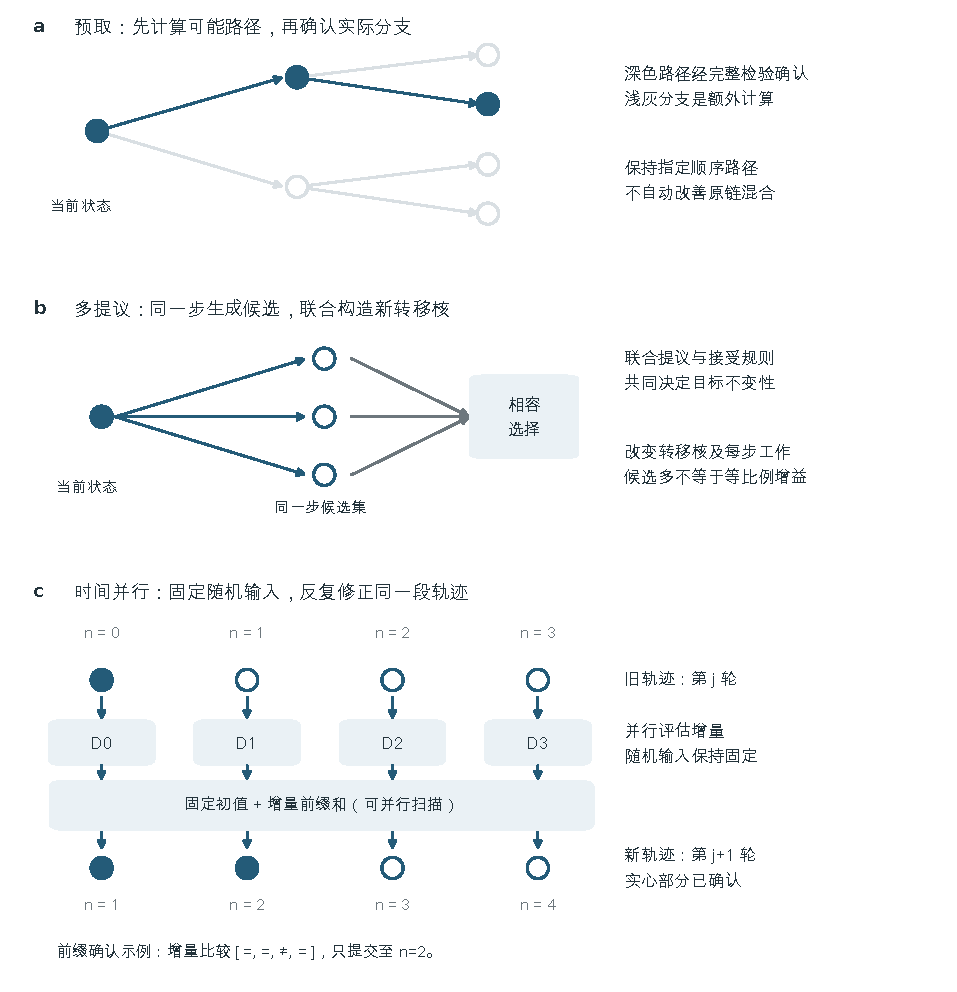
\includegraphics[width=\linewidth]{figures/fig01-mechanisms.pdf}
\caption{三种链内并行机制及其确认责任。a，预取计算可能路径，最终提交完整检验确认的分支 \cite{brockwell2006,angelino2014}。b，多提议构造新的联合转移；图中省略辅助或反向候选结构，候选不必彼此独立，下一状态也可能保留当前状态 \cite{glattholtz2024}。c，固定随机输入的 MH/Picard 窗口（$\ell=0,w=4$）。$D0$ 至 $D3$ 表示上一轮轨迹上的增量；前缀比较需要在新轨迹上再次求值。示例中的等号与不等号是相邻轮次增量的一致性比较，不是实测结果。Newton 路线将该累加步骤替换为线性化系统的仿射扫描，并仍需外层迭代 \cite{zoltowski2025,grazzi2026}。节点位置和箭头长度均无数值含义。}
\label{fig:mechanisms}
\end{figure}

这种前缀确认具有不同于连续残差阈值的作用：确认部分对应的是指定随机输入下的正确因果路径。有限长度的因果递推即使可以最终被完整恢复，也不意味着只需少量迭代；效率仍取决于每轮能确认多少状态。该文在光滑势函数、额外 Hessian 正则性以及随维度缩放的随机游走步长下，给出失配概率和并行轮数分析。在其条件下，允许的处理器规模可随 $\sqrt d$ 增长；隐藏常数与正则性参数亦需保持受控。进一步的总变差混合结论还要求强凸性与特定初始化 \cite{grazzi2026}。

初始化对轨迹求解和对统计混合的影响也不相同。该文 Proposition 1 在其强凸条件下表明，初值向远端尾部移动时，Picard 轨迹求解可趋于更快；这不等于从远离目标的初值获得可靠后验估计更容易。相反，求解器可以更快生成一段尚未进入典型区域的链。将两种收敛混称为“算法收敛”，会掩盖这一差异。

在 Newton 型 MCMC 中，接受分支的处理也不能只依据形式上的可微性。Zoltowski 等在所研究采样器中对相关 Jacobian 采用专门处理，而前向计算仍保留真实的接受检验 \cite{zoltowski2025}。局部求解残差、相同随机输入下的轨迹差与后验分布差异分别回答不同问题。若提前停止只根据数值容差输出尚未确认的轨迹，便需要额外分析其统计影响。

\subsection{并行 Langevin 的分布误差与复杂度边界}

对 Langevin 动力学，时间并行不仅可以用于恢复一个指定离散递推，也可以成为构造近似采样算法的组成部分。Anari 等通过并行 Picard 近似连续动力学，在适当的函数不等式、光滑性、初始分布及 score 精度条件下控制分布误差 \cite{anari2024}。这些结果将数值模拟误差与动力学趋近平稳分布的分析连接起来，因此比单纯轨迹求解多了一层统计保证。

理解这类定理需要同时保留误差、维度和条件数。对数 Sobolev 不等式（log-Sobolev inequality，LSI）与运输不等式在证明中的作用不同；用于控制某一离散误差的较弱条件，未必足以替代混合分析所需条件。并行查询轮数中对维度的较弱依赖，也可能伴随很大的每轮查询宽度。省略这些信息，会使理论中的“快”被误解为现实设备上的低延迟。

Zhou 和 Sugiyama 通过交错推进时间片进一步改进部分对数凹采样设定下的并行轮数，并分析有限处理器时的变化 \cite{zhou2025parallel}。其结果说明，有限硬件问题已有理论前作；实际应用所缺少的不是对处理器限制的首次认识，而是将相应界与后验几何、内存和软件开销联系起来的可靠预测。表~\ref{tab:2} 对主要保证作条件化归纳。

\begin{table}[htbp]
\centering\zihao{5}
\caption{时间并行相关成果的保证与条件}\label{tab:2}
\parbox{\linewidth}{\footnotesize “轨迹”指指定随机输入下的递推；“分布”指算法输出的概率分布。该表不是所有定理的替代，精确参数应查相应原文。}\par\smallskip
\begin{tabular}{@{}>{\raggedright\arraybackslash}p{\dimexpr0.2\linewidth-1.5\tabcolsep\relax}>{\raggedright\arraybackslash}p{\dimexpr0.25\linewidth-1.5\tabcolsep\relax}>{\raggedright\arraybackslash}p{\dimexpr0.27\linewidth-1.5\tabcolsep\relax}>{\raggedright\arraybackslash}p{\dimexpr0.28\linewidth-1.5\tabcolsep\relax}@{}}
\toprule
方法路线 & 主要控制对象 & 关键前提或机制 & 不能直接外推的结论 \\
\midrule
DEER 与光滑 Newton 序列求解 \cite{lim2024} & 数值轨迹及局部求解收敛 & 可微性、线性化系统求解及适当初值；扫描成本 & 不自动提供 MCMC 目标不变性 \\[4pt]
Newton 型 MCMC \cite{zoltowski2025} & Gibbs/MALA/固定步数 HMC 的轨迹；近似版本的经验误差 & 具体采样器适配、Jacobian 近似、容差及窗口 & 提前停止后一般后验偏差有界 \\[4pt]
精确 Online Picard \cite{grazzi2026} & MH 接受事件及已确认前缀 & 固定随机输入；复杂度定理有目标正则性和尺度条件 & 无条件的维度加速或快速混合 \\[4pt]
近似 Online Picard \cite{grazzi2026} & 接受／增量事件的失配比例 & 相邻迭代的容忍规则；命题 3 的概率控制另有前提 & 增量失配比例就是状态失配或后验函数偏差 \\[4pt]
并行 Langevin \cite{anari2024,zhou2025parallel} & 指定度量的分布误差 & 函数不等式/对数凹性、光滑性、初始化、score 与离散误差 & 任意多峰后验均有相同复杂度 \\[4pt]
可预测性与统一框架 \cite{gonzalez2025predict,gonzalez2026} & 递推稳定性、残差几何和求解迭代 & Jacobian 乘积、光滑性、一致控制及近似结构 & 负 Lyapunov 指数足以保证任意 MH 高效 \\[4pt]
PiX-MC 预印本 \cite{wei2026} & 特定成像模型下的时间平均相对 Fisher 信息 & 近端结构、score 误差及相应全局正则/矩条件 & 重建质量达标等于一般后验校准 \\[4pt]
\bottomrule
\end{tabular}
\end{table}

附录~\ref{app:theory} 将 Anari 等的过阻尼 LMC、欠阻尼 ULMC 与 Zhou 和 Sugiyama 的交错方案分别列出。这个对照带来两项具体判断：相近轮数下，ULMC 可降低每轮查询宽度；交错方案进一步减少轮数，却同时展开多个时间片，扩大查询和存储需求。在有限核心数不超过其给定阈值时，后一轮数优势会消失 \cite{anari2024,zhou2025parallel}。因此，理论上轮数更少与设备上执行更快之间，还需要核对查询并发与内存。

并行复杂度下界进一步限定了可以期待的普遍保证。Zhou、Wang 和 Sugiyama 在每轮允许多项式数量 oracle 查询的模型中，构造了高精度对数凹采样的困难实例 \cite{zhou2025lower}。其 Theorem 4.1 针对 $1$-强凸、$2$-光滑势函数，取 $\varepsilon=O(c^d)$（$0<c<1$）及所给无穷 Rényi 暖启动，得到接近线性维度的轮数下界。若把这样的精度代入附录中的上界，每轮查询数因含 $\varepsilon$ 的负幂而可能变成指数规模，已超出下界的多项式查询模型。因此两者不能直接比较；也不能将下界改述为固定精度下所有时间并行都无效。

\subsection{可预测性与应用扩展}

轨迹求解的困难可以从扰动如何沿递推传播来理解。Gonzalez 等利用 Jacobian 乘积、Lyapunov 指数和 Polyak–Łojasiewicz 条件分析非线性状态空间模型的可并行性 \cite{gonzalez2025predict}。其结果为“某些长序列为何只需较少外层迭代”提供解释，但依赖比单次观测到局部稳定更强的一致条件；收敛界中的其他常数也可能随序列长度变化。该分析不能未经处理地套用于具有不连续接受分支的任意 MH 链。

此外，更容易预测的递推不必具有更好的统计混合。例如，减小步长可能使相邻状态更接近、数值近似更可靠，却增加探索后验所需的更新次数。这提示方法选择应联合评价轨迹求解与统计效率，而不是只优化 Jacobian 近似误差或每轮残差下降。

时间并行也已进入较大规模应用。PiX-MC 将 Picard 迭代、近端似然更新、学习的 score 和退火结合用于贝叶斯成像，并在其假设下分解多个误差来源 \cite{wei2026}。其 Theorem 1 控制 $T^{-1}\int_0^T\mathrm{FI}(\mu_t\Vert\pi)\,\mathrm dt$，并进一步利用凸性讨论时间平均边缘分布；这两者均不同于末时刻总变差保证，度量转换还需额外条件。真实图像上的峰值信噪比（peak signal-to-noise ratio，PSNR）主要评价重建质量，不能单独验证后验不确定性的校准。该预印本的意义在于展示扩展方向，并不消除学习先验误差与数值误差需要分别评估的要求。

\section{现代硬件、多链基线与诊断}

\subsection{硬件适配改变算法的成本结构}

硬件的并行吞吐、内存带宽和控制流特征决定了同一数学操作的实际代价。大量形状一致的数组运算通常适合批处理，而不同链具有不同循环长度时，同步执行可能产生等待。时间并行将更多位置同时展开，有助于增加可供执行的工作，也可能使轨迹和 Jacobian 超过设备内存。因而硬件适配不能归结为“将代码放到 GPU” \cite{sountsov2026}。

数值精度也属于统计实现的一部分。后验对数密度或能量差进入 MH 接受判断，当很大的相近数值相减时，较低精度可能改变结果。并行归约和不同运算顺序也会改变舍入误差。因此，比较不同实现时应披露精度设置，并将高精度或结构化的数值核对作为必要检查，而不是假定相同公式必然产生相同接受事件 \cite{sountsov2026}。

完整工作流还受到即时编译（just-in-time compilation，JIT）和调参成本影响。编译后单次运行较快的方法，在只使用一次的模型上未必更便宜；能够重复使用同一编译结果时，其优势又可能扩大。窗口变化、模型形状变化和跨设备通信会改变这种摊销关系。因此，冷启动时间与重复运行的采样时间应分别测量，而不能仅报告较有利的一种。

\subsection{多链调参是比较基线的一部分}

多链并行不只意味着独立复制同一个默认采样器。链群可以为尺度、预条件或步长选择提供信息，但共享机制可能改变概率结构。MEADS 将广义 Hamiltonian Monte Carlo（generalized HMC，GHMC）与分折群体调参结合，利用其他折的状态构造保持相应条件目标的更新 \cite{hoffman2022}。其意义既包括自动调参，也包括对共享信息方式的约束；任意同步或异步地用全部当前状态更新各链参数，不能自动继承相同的不变性。

LAPS 将较快的未校正阶段用于预热，再转入 Metropolis 校正阶段，并通过群体统计量选择参数 \cite{robnik2026}。开启 MH 检验处理积分近似，停止群体自适应则是另一环节；原文在校正阶段完成步长调节后冻结超参数（第 2 节及第 5.1 节）。冻结后的核保持目标，并不意味着切换当时的样本立刻无初始化偏差。这种方法说明，从初始分布进入目标相关区域的成本可能主导多链总时间；其每链梯度效率仍需结合实际并行资源解释。

因此，链内或时间并行方法至少应与经过合理预热和调参的多链实现比较。仅与单链、默认参数或未经向量化的顺序实现对照，能够说明局部执行收益，却不足以回答固定硬件预算下应选哪条路线。自适应 MCMC 的经典结果同样提醒，调参并非统计上免费的操作；保证需要具体条件，不能由“每个固定参数的核都正确”直接推出 \cite{roberts2007}。

\subsection{动态 NUTS 的向量化与单链时间并行}

No-U-Turn Sampler（NUTS）依据动态路径构建与停止规则选择 HMC 的轨迹长度 \cite{hoffman2014}。相比固定积分步数的 HMC，这种控制流使不同链和不同转移可能执行不同数量的计算。将固定步数 HMC 的时间并行结果直接推广至完整 NUTS，需要处理动态路径、状态选择和随机输入等额外问题。

Dance 等使用有限状态机（finite-state machine，FSM）组织采样器的计算步骤，允许不同链按自身进度推进，减少在每个完整样本处等待最慢链的代价 \cite{dance2025}。这种方法已经展示动态采样器，包括 NUTS，能够从更合适的向量化执行中获益；与此同时，状态机和掩码等开销也可能导致部分问题变慢。它解决的是多链控制流调度，与一次求解同一条链多个未来采样位置的时间并行不同。

上述区分使动态 NUTS 的研究问题更具体：需要判断沿链长或积分过程引入并行求解后，是否仍实现所需转移核，以及节省的计算是否超过动态构建、同步和额外存储。已有 FSM 和固定步数 HMC 方法应成为比较对象，而非被描述成尚无人处理动态采样器。

\subsection{许多短链需要相应诊断}

当硬件允许同时运行大量链时，总样本量可以迅速增加，但许多短链可能共同保留初始化影响。增加链数有助于降低某些随机误差，却不自动消除共同的非平稳偏差。Nested R-hat 将共享初值、条件于该初值独立运行的若干链组织为 superchain，并利用不同层次的变异评估短链收敛 \cite{margossian2025}。这为大量短链提供了专门工具，而不要求简单沿用少数长链的经验。

该诊断仍有明确边界。较小的诊断值不构成任意目标上收敛或无偏的证明；组数选择、调参阶段以及较难发现的模式仍需谨慎处理 \cite{margossian2025}。对时间并行近似输出，还应额外检查数值求解误差。一个诊断器可能发现链间不一致，却未必发现所有链都受到相同算法近似的影响。因此，应把轨迹求解诊断、初始化诊断与估计 MCSE 看作相互补充的证据。

\section{加速证据与比较原则}

\subsection{文献中的速度比对应不同问题}

现有研究使用的效率指标包括并行轮数、梯度调用次数、谱隙、ESS、重建质量及墙钟时间。这些量分别衡量算法或执行过程的不同方面。表~\ref{tab:3} 保留具有代表性的数值结果，同时给出其预算和解释范围；它不构成横向性能排名，也不是本文的新实验。

\begin{table}[htbp]
\centering\zihao{5}
\caption{代表性加速证据及计量条件}\label{tab:3}
\parbox{\linewidth}{\footnotesize 数值摘自相应原论文；“倍数”须与同一行的比较对象一起理解。没有报告统一的不确定区间时，不补造跨研究合并估计。}\par\smallskip
\begin{tabular}{@{}>{\raggedright\arraybackslash}p{\dimexpr0.2\linewidth-1.5\tabcolsep\relax}>{\raggedright\arraybackslash}p{\dimexpr0.25\linewidth-1.5\tabcolsep\relax}>{\raggedright\arraybackslash}p{\dimexpr0.29\linewidth-1.5\tabcolsep\relax}>{\raggedright\arraybackslash}p{\dimexpr0.26\linewidth-1.5\tabcolsep\relax}@{}}
\toprule
来源及实验 & 原文报告的结果 & 预算与比较条件 & 可支持的判断 \\
\midrule
预测性预取的高斯混合例子 \cite{angelino2014} & 64 个 worker 时，预热段约 16.8 倍；50,000 步全程约 5.8 倍 & 8 分量、8 维、100 万观测；预热段为 9,575 步；旧硬件/网络环境 & 路径预测的收益随阶段变化，不能用最高短时倍数代表全程 \\[4pt]
现代硬件章的 HMC/NUTS 基准 \cite{sountsov2026} & GPU HMC 2.4 s，GPU NUTS 4.3 s & 稀疏 logistic 回归；64 链各 1000 步；P100；手工预调参未计时 & 说明所选模型的采样阶段差异，不能外推完整自动化推断成本 \\[4pt]
Newton 型 MALA 及其窗口版本 \cite{zoltowski2025} & 部分小批量约 20–30 倍；768 维窗口例子超过 3 倍 & 主要计时排除 JIT；后者为 4 链、每链 4096 步、最优窗口 256；大批量可能变慢或内存不足 & 时间并行存在有效区间，也存在资源竞争和内存限制 \\[4pt]
Online Picard 的昂贵常微分方程（ODE）似然 \cite{grazzi2026} & 理想轮数增益约 4.37，实际墙钟增益约 2.52 倍 & 14 维模型、Mac M3、8 个并行计算位置 & 并行开销会缩小理论或理想执行收益 \\[4pt]
LAPS 多链比较 \cite{robnik2026} & 原表 1 在其任务上约 2–20 倍的每链梯度效率改善 & 4096 链；坐标二阶矩标准化平方偏差的最大值降至 0.01 & 支持所测预算下的梯度效率，不直接提供跨设备墙钟倍数 \\[4pt]
FSM 向量化 NUTS \cite{dance2025} & 四个实际模型的 ESS/s 比为 1.5、3.5、1.2、0.8 & A100/JAX；128 链各 1000 样本；400 步预热调参 & 动态控制流调度能有收益，也存在 ESS/s 下降的案例 \\[4pt]
PiX-MC 的三维 CT 例子 \cite{wei2026} & 同配方串行/并行达到参考 PSNR 的时间为 116\(\to\)37 min、28\(\to\)9 min，约 3.1 倍 & 并行使用 8 张 GPU，串行 1 张；最高约 50 倍还跨越算法与 PSNR 阈值（30.5/32.5 dB） & 配对结果支持所给资源下的执行收益；50 倍不是同精度下的纯并行加速 \\[4pt]
\bottomrule
\end{tabular}
\end{table}

这些结果共同支持一个条件化判断：链内并行具有实际价值，但收益强烈依赖模型、初始化、执行阶段和资源配置。不同报告的差异可能来自方法机制，也可能来自硬件数量、编译摊销、参数调优或参考精度。缺少共同协议时，不宜用最大速度比判断算法优劣。附录~\ref{app:evidence} 补充表中组合案例的原始图表位置、模型对应和不确定性口径。

\subsection{共同精度目标先于共同样本数}

若两个实现产生相同的固定随机输入轨迹，在核对数值等价后，用相同步数比较执行时间具有直接含义。若它们使用不同转移核，或一个输出为提前停止的近似轨迹，相同原始样本数就不再代表相同推断精度。此时需针对预先指定的函数或分布度量比较误差，再解释时间差。

参考分布的可靠性是这一比较的一部分。解析高斯模型允许直接检验若干期望及分布性质，适合分离实现误差与 Monte Carlo 波动；复杂后验往往只能采用较长、独立的参考计算。后者仍可能混合不足，其估计不确定性应进入解释。基于有限参考样本的分布距离下降提供有用证据，但不足以证明所有后验函数均已准确，或尾部和模式权重均得到恢复。

对图像等应用任务，还需区分决策质量与分布质量。更快达到某一重建指标可以是有意义的应用收益，但若论文声称改进 posterior sampling，就应进一步评价不确定性、覆盖率或适当分布误差。不同目标可以并列报告，却不能相互替代。

以 German Credit logistic 回归为例，Zoltowski 等在单张 H100、相同步长的 MALA 上同时改变链数与链长。充分数值收敛后的准 Newton 执行在部分小批量下更快，且相对于 NUTS 参考样本的最大均值差异（maximum mean discrepancy，MMD）与顺序执行接近；链数增至 32 时收益反转，原文 Fig. 4 的部分配置还采用插值计时 \cite{zoltowski2025}。据此可以支持该设置下的轨迹执行收益及共同 MMD 代理下的资源取舍，不能直接断言式（5）已经达标。提前停止至 8 次 Newton 迭代的案例又是另一层结论：相近 MMD 是近似输出的经验支持，不能继承充分收敛时的轨迹等价。

若研究者需要比较特定系数与风险预测，可事先选择 $\mathcal F=\{\theta_k,\theta_k^2,\Pr(Y_{\rm new}=1\mid\theta,z_*)\}$，将关注的 $k$、固定协变量 $z_*$、尺度 $s_f$ 和误差阈值一并写入协议；这是本文给出的任务示例，并非上述原论文已测量的函数集合。解析真值可用于独立重复的 MSE 评估；只有独立参考时，须同时报告参照误差，并避免将待评估样本复用于参考；只有 ESS、MCSE 或 $\widehat R$ 等诊断时，则将结论限定为诊断代理下的效率。三种证据均可用来缩小配置选择范围，但只有与预设目标相符的误差证据才能支持“达到共同精度”。

昂贵且无梯度的 ODE 似然提供另一种情境。若目标是保留指定随机游走链且可利用 8 个计算位置，Online Picard 的配对实验支持所测模型上约 2.52 倍的墙钟收益；若目标改为同预算下最快获得准确后验期望，则还要检验原核的混合并与可用的替代核比较 \cite{grazzi2026}。这说明方法选择可以先利用已确认的执行收益筛选候选，再补足任务相关的统计比较。

\subsection{完整成本与失败区间}

公平比较应预先明确约束的是处理器数量、设备数量、内存、墙钟时间还是总计算工作。多卡算法相对单卡缩短时间，回答的是扩展资源后的延迟问题；相同设备预算下比较不同并行轴，则回答资源分配问题。两者均有价值，但不是同一个实验。

预热、调参和编译的处理方式同样需要一致。若某方法使用额外的搜索或先验运行选定配置，该成本应披露；如果讨论重复使用同一模型时的摊销收益，也应同时给出冷启动场景。对异步设备计时，应使用能够反映实际任务完成的同步测量，避免把发起计算的时间当作完成计算的时间。

失败配置应与成功配置共同定义适用范围。高维 Jacobian 引起的内存不足、较大链数下时间并行的收益反转，以及动态控制流实现的额外开销，均会影响用户的选择，不能只作为实现细节隐藏 \cite{zoltowski2025,dance2025}。除平均运行时间外，报告独立重复间的变异、配置失败率及所需内存，能够帮助区分稳定收益与偶然有利的参数组合。

\section{讨论与开放问题}

\subsection{从数值残差到后验函数误差}

时间并行带来的一个核心问题是，何时可以停止轨迹求解。完整确认原递推与提前停止输出近似轨迹的证明责任不同：前者主要需要确认执行等价性，后者还需控制近似对推断的影响。已有 Picard 失配分析、Langevin 分布误差理论及 Newton 型方法的经验比较提供了不同层次的答案，但尚不能统一为适用于实际 MH 后验的廉价误差证书。

核扰动理论已经说明，局部近似误差如何影响分布误差取决于原链的收敛性质 \cite{mitrophanov2005,alquier2016}。为说明这一关系，考虑齐次 Markov 核 $K$ 及其近似 $\widetilde K$，定义总变差为 $\|\mu-\nu\|_{\mathrm{TV}}=\sup_A|\mu(A)-\nu(A)|$。若对所有概率分布满足

\begin{equation}
\begin{aligned}
\|\mu K-\nu K\|_{\mathrm{TV}}&\leq\rho\|\mu-\nu\|_{\mathrm{TV}},\qquad \rho<1,\\
\sup_x\|K(x,\cdot)-\widetilde K(x,\cdot)\|_{\mathrm{TV}}&\leq\delta.
\end{aligned}
\label{eq:11}
\end{equation}

则由三角不等式递推可得，对具有相同初始分布的两个过程，

\begin{equation}
\|\mu\widetilde K^{\,n}-\mu K^n\|_{\mathrm{TV}}
\leq \delta\sum_{i=0}^{n-1}\rho^i
\leq\frac{\delta}{1-\rho}
\label{eq:12}
\end{equation}

式（12）只是强收缩条件下的说明性推导，不是本文针对时间并行的新定理，也不代表所有 MCMC 都满足式（11）。它说明即使单步误差较小，较慢的混合仍可能放大分布偏差。一般情况下，相关理论需要多步收缩、漂移或其他稳定性条件，而这些量未必能够低成本估计。

这一分布界尚不是式（5）的 MSE 界。对有界函数，令 $\operatorname{osc}(f)=\sup f-\inf f$，按本文的总变差约定有
\[
|\mu\widetilde K^{\,n}f-\pi f|
\leq\operatorname{osc}(f)\!\left\{\delta\sum_{i=0}^{n-1}\rho^i
+\|\mu K^n-\pi\|_{\mathrm{TV}}\right\}.
\]
右侧分别反映近似核误差与基准链的初始化、混合误差。对保留时刻作平均可控制样本均值的偏差，却仍未控制相关轨迹造成的估计方差。坐标均值、二阶矩等无界函数还需要相应矩控制或加权范数条件，不能仅凭总变差小就获得统一函数误差界。图~\ref{fig:evidence} 标明了这些连接所需的额外条件。

\begin{figure}[htbp]
\centering
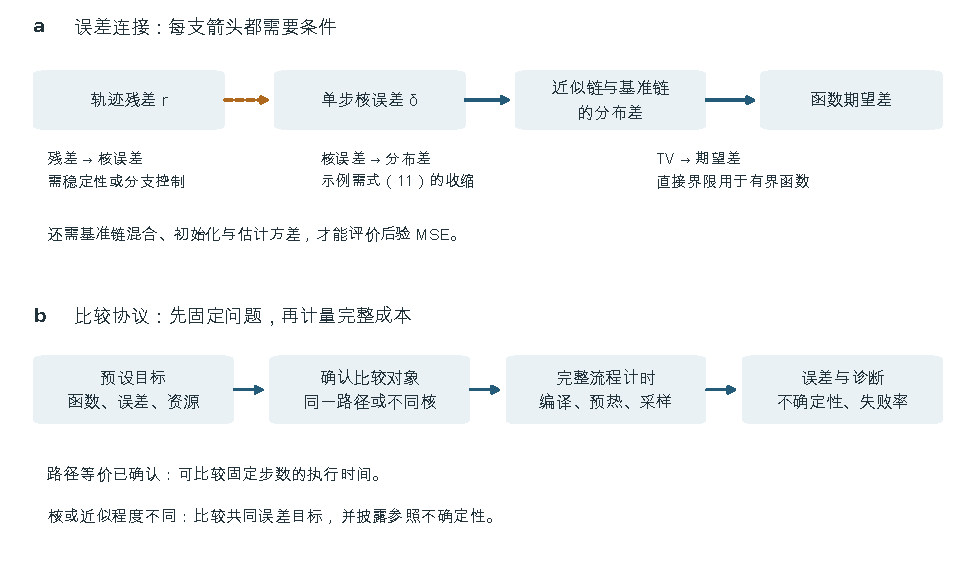
\includegraphics[width=\linewidth]{figures/fig02-evidence-workflow.pdf}
\caption{从数值求解到推断成本的证据链。a，橙色虚线标出尚需针对具体算法建立的残差到核误差连接；蓝色实线同样带有条件，并不表示任意 MH 均满足式（11）。有界函数的期望差仍需与初始化、混合及估计方差区分 \cite{mitrophanov2005,alquier2016}。b，依据已有预算评价与硬件讨论整理的比较协议 \cite{angelino2016,sountsov2026}。不同证据等级决定可以声称的收益范围；图中没有经验速度比或实验测量。}
\label{fig:evidence}
\end{figure}

将这一思路转化为实用停止准则还有两道缺口。首先，轨迹残差或接受／增量事件失配率需要转化为适当的核或函数误差。Grazzi 和 Zanella 第 5 节中实际容忍的是相邻 Picard 轮次的增量不一致比例，Proposition 3 则在所给条件下控制相对精确递推的增量失配概率；两者均不能直接解释为整条轨迹的状态失配率。其次，采用窗口历史、自适应容差或状态相关停止的输出，未必对应上述齐次核模型。可先在有明确收缩或可控混合的模型上建立函数导向的保证，再检验其保守程度与计算成本。

\subsection{有限资源下的并行轴选择}

硬件章、时间并行实验和有限处理器理论已经证明，链数、窗口与其他并行维度之间存在取舍 \cite{sountsov2026,zoltowski2025,zhou2025parallel}。因此，开放问题不宜表述为“首次考虑资源分配”。更具体的问题是：能否利用短时探测、模型结构和误差需求，在受限内存与设备预算下选择配置，并在多类后验中持续优于简单固定配置？

这一问题需要区分数值调度与采样核自适应。若配置只改变求解同一递推的执行次序，且最终保留准确路径，其统计负担相对明确；若同时改变步长、提议、近似容差或停止规则，便可能改变核或输出分布。选择器的探测开销、重新编译及调参成本也必须计入性能，而不能只比较配置选定后的最短一次运行。

评价这种机制可先采用范围有限的基准：可解析高斯目标用于控制维度和条件数，一个非高斯分层后验检验几何适配，一个昂贵似然问题检验并行开销摊销，多峰问题作为单独压力测试。该设计是后续验证建议，本文没有运行这些实验。其目的不是用少量模型证明普遍最优，而是识别选择规则失效的条件，并比较其相对固定调优和多链基线的增量价值。

\subsection{动态采样器、可预测性与混合}

动态 NUTS 的挑战来自路径构建、停止与状态选择的耦合。已有 FSM 方法减少多链间的等待，固定步数 HMC 的时间并行则处理较规则的递推；组合两者能否带来净收益仍需逐项验证。一个保留目标分布但明显增加预热或内存成本的实现，不一定优于现有多链方案。相应研究应先确认概率构造，再比较完整推断成本。

可预测性提供了另一条研究线索：数值递推越稳定，可能越容易用较少并行迭代求解；但统计上有益的大步探索或跨模式移动，又可能降低路径预测的可靠性 \cite{gonzalez2025predict,gonzalez2026}。现有理论已开始刻画前一关系，后一关系仍需要结合具体采样核分析。值得检验的不是单个局部指标能否与运行时间相关，而是它在改变步长、预条件和目标几何后，是否仍能预测达到共同误差所需的时间。

\subsection{多提议极限与可检验的研究问题}

多提议研究说明，增加候选数量可能受核效率限制，也可能改变近似偏差或趋向某个不同的极限核 \cite{pozza2025,glattholtz2026}。因而有限提议数的选择不仅是吞吐调优：还涉及目标维度、提议尺度、接受规则及极限核本身的混合。用无限资源极限解释机制有理论价值，但实际推荐必须回到有限计算和内存。

表~\ref{tab:4} 汇总本文覆盖范围内的研究问题。提前停止偏差已见于 Grazzi 和 Zanella 第 5 节；长链与多链资源分配、调参及 NUTS 扩展已见于 Zoltowski 等第 6 节；核与目标的可预测性刻画见 Gonzalez 等的讨论；极限核混合、维度与提议尺度、偏差诊断见 Mad Props 第 7 节第 1 至 4 项 \cite{grazzi2026,zoltowski2025,gonzalez2025predict,glattholtz2026}。本文进一步把这些议程收束到指定函数的误差证书、计入探测和编译的配置收益，以及共同预算下的验证。它们不是经过穷尽检索确认的全领域空白。

\begin{table}[htbp]
\centering\zihao{5}
\caption{开放问题及其最小验证方向}\label{tab:4}
\begin{tabular}{@{}>{\raggedright\arraybackslash}p{\dimexpr0.17\linewidth-1.5\tabcolsep\relax}>{\raggedright\arraybackslash}p{\dimexpr0.25\linewidth-1.5\tabcolsep\relax}>{\raggedright\arraybackslash}p{\dimexpr0.3\linewidth-1.5\tabcolsep\relax}>{\raggedright\arraybackslash}p{\dimexpr0.28\linewidth-1.5\tabcolsep\relax}@{}}
\toprule
问题 & 已有基础 & 仍需回答的具体问题 & 有区分力的验证 \\
\midrule
提前停止与估计误差 & 增量失配分析、近似核理论、特定 Langevin 误差界 & 可计算残差如何控制指定后验函数偏差？ & 在有真值或可控混合的模型上检验证书覆盖与计算成本 \\[4pt]
有限资源选择 & 并行轴比较、有限处理器分析、窗口化 & 在线选择是否在计入探测/编译后仍有收益？ & 同设备、同内存、同精度，与固定调优和简单搜索比较 \\[4pt]
动态 NUTS 时间并行 & 固定步数 HMC、FSM 多链调度 & 动态停止与路径选择能否正确并行且产生净收益？ & 先核对核构造与随机输入，再做包含预热的对照 \\[4pt]
可预测性与统计混合 & Lyapunov/残差几何、统一序列框架 & 容易并行的核是否也能较快获得有效后验信息？ & 联合改变步长、几何与多峰程度，同时测求解成本及估计误差 \\[4pt]
有限多提议数量 & 核比较上界、无限提议极限 & 提议数和维度共同增长时的偏差、混合与成本如何变化？ & 固定接受规则，联合扫描维度、尺度与提议数，并保持预算可比 \\[4pt]
\bottomrule
\end{tabular}
\end{table}

\subsection{综述的适用范围}

本文的组织原则适用于比较所选链内与时间并行方法，但不能替代所有并行贝叶斯领域的全面回顾。对于异步 Gibbs、数据分片近似或粒子系统，误差来源与依赖结构可能不同，需要相应专门理论。前沿中的预印本结论亦应按实际版本引用，不能假定其已经获得与正式发表文献相同的验证。

跨文献综合还受到实验异质性的限制。不同目标、初始化、实现语言、硬件和误差代理，使现有速度比难以直接合并；本文未通过统一代码重新测量它们。因此，本文能够支持的是方法适用条件和比较原则，而非普遍最优的算法推荐。正式基准若发现不同的收益区间，应据结果修订选择建议，而不是要求实验服从既有分类。

\section{结论}

链内与时间并行 MCMC 已形成多种具有不同统计含义的路线。预取可以通过最终路径确认保持指定顺序执行，多提议依赖新的核构造，而 Picard/Newton 方法通过并行求解轨迹重新分配顺序计算。它们共同拓展了并行硬件的利用方式，但减少执行深度、保持目标不变和获得准确后验估计并不是同一结论。

比较这些方法时，首先应明确目标函数或分布误差，再将理论条件、总工作量、内存和完整工作流时间放在同一框架中。现有理论及正负实验结果支持按目标几何、计算密度和资源预算选择方法；它们尚不足以给出独立于任务的速度排名。将可计算的数值误差连接到后验估计误差，并在有限硬件上验证配置选择，是进一步提高时间并行实用性的关键方向。

\clearpage
\appendix
\section{代表性并行 Langevin 定理的参数对照}\label{app:theory}

为给出可比较的切片，表~\ref{tab:theory} 采用 $V$ 为 $\alpha$-强凸、$\beta$-光滑的共同子情形，记 $\kappa=\beta/\alpha$。位置初始化为 $\mu_0=N(x_*,\beta^{-1}I_d)$，其中 $x_*$ 为势函数极小点；ULMC 另以独立 $N(0,I_d)$ 初始化动量。求得 $x_*$ 的成本未包括在下列采样轮数中。误差参数为 $\varepsilon$，统一点态梯度近似误差记为 $\delta_s$。采用 $\log_+z=\max\{1,\log z\}$ 表示量级比较中的截断对数，整数参数向上取整；$\widetilde O$、$\widetilde\Theta$ 保留原文隐藏对数因子的约定，不能据此删除条件数依赖。

\begin{table}[htbp]
\centering\zihao{5}
\caption{共同强对数凹子情形下的输出保证、查询和存储}\label{tab:theory}
\begin{tabular}{@{}>{\raggedright\arraybackslash}p{\dimexpr0.24\linewidth-1.5\tabcolsep\relax}>{\raggedright\arraybackslash}p{\dimexpr0.24\linewidth-1.5\tabcolsep\relax}>{\raggedright\arraybackslash}p{\dimexpr0.25\linewidth-1.5\tabcolsep\relax}>{\raggedright\arraybackslash}p{\dimexpr0.27\linewidth-1.5\tabcolsep\relax}@{}}
\toprule
结果与定位 & 输出及梯度误差 & 总轮数 $R$；每轮查询宽度 $Q$ & 同时保留的状态网格 \\
\midrule
并行 LMC \cite{anari2024}，Corollary 14 & $\mathrm{KL}\leq2\varepsilon^2$，$\mathrm{TV}\leq\varepsilon$；$\delta_s\leq2\sqrt\alpha\varepsilon$ & $R=NK$；$Q=M=O(\max\{\kappa d/\varepsilon^2,\kappa^2\})$ & 每次处理一个时间片，$O(dM)$ 个标量 \\[5pt]
并行 ULMC \cite{anari2024}，Theorem 15 & 位置边缘 $\mathrm{TV}\leq\varepsilon$；$\delta_s\leq\widetilde O(\sqrt\alpha\varepsilon/\sqrt{\log d})$ & $R=NK$；$Q=M=\widetilde\Theta(\sqrt{\kappa d}/\varepsilon)$ & 每片的位置和动量，$O(dM)$ 个标量 \\[5pt]
交错 Picard \cite{zhou2025parallel}，Theorem 4.2、Corollary 4.3 & $\mathrm{KL}\leq8\varepsilon^2$，$\mathrm{TV}\leq2\varepsilon$；$\delta_s\leq0.2\sqrt\alpha\varepsilon$ & $R=N+(N+J)H$；$Q\leq MN$，$M=O(\kappa d/\varepsilon^2)$ & 同时展开多个时间片，$O(dMN)$ 个标量 \\[5pt]
\bottomrule
\end{tabular}
\par\smallskip
\parbox{\linewidth}{\footnotesize 网格存储由算法中同时保留的状态数计数，仅用于显示宽度代价，不是实测峰值内存；不含实现缓冲区、模型或自动微分开销。$N$ 为时间片数，$K$ 为片内 Picard 轮数，$J$ 为交错方向轮数，$H$ 对应 Zhou 和 Sugiyama 原文的内循环参数 $P$，与硬件处理器数不同。}
\end{table}

LMC 取 $h=1/(10\beta)$，$N=O\{\kappa\log_+(d\log_+\kappa/\varepsilon^2)\}$、$K=O(\log_+M)$；原文给出的轮数简写为 $\widetilde O\{\kappa\log^2(d/\varepsilon^2)\}$。该文更一般的 Theorem 13 只要求 LSI 常数 $\alpha$、$\beta$-光滑及有限初始 $D_0=\mathrm{KL}(\mu_0\Vert\pi)$，并要求 $Nh\geq\alpha^{-1}\log(2D_0/\varepsilon^2)$ 等条件。因此，表中的强凸性是比较所选子情形，不能倒过来宣称该 LMC 定理只适用于强凸目标。

ULMC 取 $h=\Theta(\beta^{-1/2})$、$K=\Theta\{\log_+(\kappa d/\varepsilon^2)\}$、$N=\widetilde\Theta\{\kappa\log(d/\varepsilon^2)\}$。其轮数同为 $\widetilde\Theta\{\kappa\log^2(d/\varepsilon^2)\}$，但每轮查询宽度的维度与精度依赖更小；这里的定理输出是 TV 保证，不能补写成 LMC 行的同一 KL 保证。

交错方案取 $h=1/(10\beta)$、$N=O\{\kappa\log_+(d\log_+\kappa/\varepsilon^2)\}$、$H=O(\log_+\kappa)$，以及 $J-N=O\{\log_+(\kappa^2d\log_+\kappa/\varepsilon^2)\}$，得到原文简写的 $R=\widetilde O\{\kappa\log(d/\varepsilon^2)\}$ 和 $Q=\widetilde O\{\kappa^2d\varepsilon^{-2}\log(d/\varepsilon^2)\}$。若要求共同 TV 阈值 $\eta$，前两行可令 $\varepsilon=\eta$，第三行需令 $\varepsilon=\eta/2$，相应查询与 score 精度也随之变化。

有限硬件下，Zhou 和 Sugiyama 的 Remark 4.6 给出核心数为 $\ell$ 时的量级 $\widetilde O\{\kappa^2d(\varepsilon^2\ell)^{-1}\log^2(d/\varepsilon^2)\}$，并指出在 $\ell\leq\kappa d/\varepsilon^2$ 区域不再改善其所比较的既有轮数界。该有限核心表达不能随 $\ell\to\infty$ 外推到低于自身顺序依赖轮数 $R$；它也未计入同步、传输与设备内存。查询复杂度的取舍因此是选择候选方案的理论依据，尚不是硬件速度预测。

\section{定量摘录的任务与口径索引}\label{app:evidence}

表~\ref{tab:3} 的 Newton/MALA 小批量结果来自 Zoltowski 等第 5.2 节、Figs. 3--4，目标为 German Credit 的 logistic 回归，默认单张 H100，$B\in\{1,2,4,8,16,32\}$，链长 1K 至 64K；Fig. 3 的速度比报告 20 个种子的 90\% 区间，而迭代数面板使用 60\% 区间。768 维结果来自第 5.5 节、Fig. 7，为 IMDB 嵌入上的另一项 logistic 回归任务。计时排除 JIT，主表中的 20--30 倍并非所有小批量配置的保证 \cite{zoltowski2025}。

LAPS 的函数为 $x_i^2$，其原文式（12）定义 $b_t^2[f]=\{\mathbb E_{\rho_t}f-\mathbb E_\pi f\}^2/\operatorname{Var}_\pi(f)$。Table 1 在 4096 链下比较 $\max_i b_t^2[x_i^2]$ 降至 0.01 的每链梯度数；Table 2 在 256 链下改用 $d^{-1}\sum_i b_t^2[x_i^2]$，并分别列总梯度数和每链数。它们是平方偏差指标，不能当作已经包含方差的 MSE。高斯任务使用解析参照，其他任务采用长 NUTS 运行；原表另标注随机波动率任务的既有基线数值在前作表、图间不一致，本文不重新合并该点估计 \cite{robnik2026}。

FSM 的四个 NUTS 比值依次对应 Predator Prey、Google Stock、German Credit 和 Biochemical Oxygen Demand，定位为 Dance 等第 7.4 节、Table 1；其中 0.8 倍表示 ESS/s 下降，而非时间缩短 20\% \cite{dance2025}。硬件章的 HMC/NUTS 时间定位为第 21.4.3 节、Table 21.1 \cite{sountsov2026}。Online Picard 的 ODE 应用定位为第 6.8 节及补充材料 G 节 \cite{grazzi2026}。PiX-MC 的配对时间定位为 Fig. 9 及其后讨论；116/37 和 28/9 均约为 3.1，但其多卡条件与 PSNR 目标必须随数值一同保留 \cite{wei2026}。

\clearpage
\begin{thebibliography}{99}\zihao{5}\raggedright
\setlength{\itemsep}{4pt}
\bibitem{angelino2016} Angelino E., Johnson M.J., Adams R.P.
\href{https://arxiv.org/abs/1602.05221v2}{Patterns of Scalable Bayesian Inference}.
arXiv:1602.05221（预印本）, 2016.

\bibitem{sountsov2026} Sountsov P., Carroll C., Hoffman M.D.
\href{https://doi.org/10.1201/9781003453420-21}{Running Markov Chain Monte Carlo on Modern Hardware and Software}.
Handbook of Markov Chain Monte Carlo, 2nd ed., Chapter 21. CRC Press, 2026: 569–590.

\bibitem{bardenet2017} Bardenet R., Doucet A., Holmes C.
\href{https://jmlr.org/papers/v18/15-205.html}{On Markov chain Monte Carlo methods for tall data}.
Journal of Machine Learning Research, 2017, 18(47): 1–43.

\bibitem{robert2018} Robert C.P., Elvira V., Tawn N., et al.
\href{https://wires.onlinelibrary.wiley.com/doi/10.1002/wics.1435}{Accelerating MCMC algorithms}.
WIREs Computational Statistics, 2018, 10(5): e1435.

\bibitem{brockwell2006} Brockwell A.E.
\href{https://doi.org/10.1198/106186006X100579}{Parallel Markov chain Monte Carlo Simulation by Pre-Fetching}.
Journal of Computational and Graphical Statistics, 2006, 15(1): 246–261.

\bibitem{angelino2014} Angelino E., Kohler E., Waterland A., et al.
\href{https://arxiv.org/abs/1403.7265v1}{Accelerating MCMC via Parallel Predictive Prefetching}.
arXiv:1403.7265（预印本）, 2014.

\bibitem{calderhead2014} Calderhead B.
\href{https://doi.org/10.1073/pnas.1408184111}{A general construction for parallelizing Metropolis–Hastings algorithms}.
Proceedings of the National Academy of Sciences, 2014, 111(49): 17408–17413.

\bibitem{glattholtz2024} Glatt-Holtz N.E., Holbrook A.J., Krometis J.A., et al.
\href{https://doi.org/10.1093/imatrm/tnae004}{Parallel MCMC algorithms: theoretical foundations, algorithm design, case studies}.
Transactions of Mathematics and Its Applications, 2024, 8(2): tnae004.

\bibitem{anari2024} Anari N., Chewi S., Vuong T.D.
\href{https://proceedings.mlr.press/v247/anari24a.html}{Fast parallel sampling under isoperimetry}.
Proceedings of Thirty Seventh Conference on Learning Theory, 2024, 247: 161–185.

\bibitem{zoltowski2025} Zoltowski D.M., Wu S., Gonzalez X., et al.
\href{https://proceedings.nips.cc/paper\_files/paper/2025/hash/202886ee1c9ca735cb5bff3a00a69883-Abstract-Conference.html}{Parallelizing MCMC Across the Sequence Length}.
Advances in Neural Information Processing Systems, 2025, 38.

\bibitem{grazzi2026} Grazzi S., Zanella G.
\href{https://doi.org/10.1093/biomet/asag022}{Parallel computations for Metropolis Markov chains with Picard maps}.
Biometrika, 2026, 113(2): asag022.

\bibitem{gonzalez2026} Gonzalez X., Buchanan E.K., Lee H.D., et al.
\href{https://openreview.net/forum?id=fw6GgAIGur}{A Unifying Framework for Parallelizing Sequential Models with Linear Dynamical Systems}.
Transactions on Machine Learning Research, 2026.

\bibitem{gonzalez2025predict} Gonzalez X., Kozachkov L., Zoltowski D.M., et al.
\href{https://arxiv.org/abs/2508.16817v4}{Predictability Enables Parallelization of Nonlinear State Space Models}.
Advances in Neural Information Processing Systems, 2025.

\bibitem{zhou2025parallel} Zhou H., Sugiyama M.
\href{https://proceedings.mlr.press/v267/zhou25x.html}{Parallel Simulation for Log-concave Sampling and Score-based Diffusion Models}.
Proceedings of the 42nd International Conference on Machine Learning, 2025, 267: 79192–79225.

\bibitem{pozza2025} Pozza F., Zanella G.
\href{https://doi.org/10.1093/biomet/asaf019}{On the fundamental limitations of multi-proposal Markov chain Monte Carlo algorithms}.
Biometrika, 2025, 112(2): asaf019.

\bibitem{glattholtz2026} Glatt-Holtz N.E., Holbrook A.J., Krometis J.A., et al.
\href{https://arxiv.org/abs/2605.21899v1}{Mad Props: Parallelism in Markov Chain Monte Carlo Through the Lens of the Infinite Proposal Limit}.
arXiv:2605.21899（预印本）, 2026.

\bibitem{lim2024} Lim Y.H., Zhu Q., Selfridge J., et al.
\href{https://proceedings.iclr.cc/paper\_files/paper/2024/hash/f3bfbd65743e60c685a3845bd61ce15f-Abstract-Conference.html}{Parallelizing non-linear sequential models over the sequence length}.
International Conference on Learning Representations, 2024.

\bibitem{wei2026} Wei D., Bell E., Guo W., et al.
\href{https://arxiv.org/abs/2608.17666v1}{Picard Proximal Monte Carlo for Parallel Bayesian Imaging with Score-Based Generative Priors}.
arXiv:2608.17666（预印本）, 2026.

\bibitem{zhou2025lower} Zhou H., Wang B., Sugiyama M.
\href{https://arxiv.org/abs/2408.13045v2}{The Adaptive Complexity of Parallelized Log-concave Sampling}.
International Conference on Learning Representations, 2025.

\bibitem{hoffman2022} Hoffman M.D., Sountsov P.
\href{https://proceedings.mlr.press/v151/hoffman22a.html}{Tuning-Free Generalized Hamiltonian Monte Carlo}.
Proceedings of The 25th International Conference on Artificial Intelligence and Statistics, 2022, 151: 7799–7813.

\bibitem{robnik2026} Robnik J., Seljak U.
\href{https://proceedings.mlr.press/v300/robnik26a.html}{Faster Parallel MCMC: Metropolis Adjustment Is Best Served Warm}.
Proceedings of the 29th International Conference on Artificial Intelligence and Statistics, 2026, 300: 2719–2727.

\bibitem{roberts2007} Roberts G.O., Rosenthal J.S.
\href{https://doi.org/10.1239/jap/1183667414}{Coupling and ergodicity of adaptive Markov chain Monte Carlo algorithms}.
Journal of Applied Probability, 2007, 44(2): 458–475.

\bibitem{hoffman2014} Hoffman M.D., Gelman A.
\href{https://jmlr.org/papers/v15/hoffman14a.html}{The No-U-Turn Sampler: Adaptively Setting Path Lengths in Hamiltonian Monte Carlo}.
Journal of Machine Learning Research, 2014, 15(47): 1593–1623.

\bibitem{dance2025} Dance H., Glaser P., Orbanz P., et al.
\href{https://proceedings.mlr.press/v267/dance25a.html}{Efficiently Vectorized MCMC on Modern Accelerators}.
Proceedings of the 42nd International Conference on Machine Learning, 2025, 267: 12436–12458.

\bibitem{margossian2025} Margossian C.C., Hoffman M.D., Sountsov P., et al.
\href{https://doi.org/10.1214/24-BA1453}{Nested R-hat: Assessing the Convergence of Markov Chain Monte Carlo When Running Many Short Chains}.
Bayesian Analysis, 2025, 20(4): 1587–1614.

\bibitem{mitrophanov2005} Mitrophanov A.Yu.
\href{https://www.cambridge.org/core/journals/journal-of-applied-probability/article/sensitivity-and-convergence-of-uniformly-ergodic-markov-chains/26A9854BCB8D103B3A63A9B272616EC0}{Sensitivity and convergence of uniformly ergodic Markov chains}.
Journal of Applied Probability, 2005, 42(4): 1003–1014.

\bibitem{alquier2016} Alquier P., Friel N., Everitt R., et al.
\href{https://link.springer.com/article/10.1007/s11222-014-9521-x}{Noisy Monte Carlo: convergence of Markov chains with approximate transition kernels}.
Statistics and Computing, 2016, 26(1–2): 29–47.

\end{thebibliography}
\end{document}
